% !TEX root = smc_bandits.tex
We here evaluate non-stationary, contextual, binary reward bandits.
We resort to the logistic reward function described in Equation~\eqref{eq:logistic_rewards},
with time-varying, latent parameter dynamics as described in the following scenarios:
\begin{equation}
\text{Scenario C}
\begin{cases}
\vspace*{1ex}
p(\theta_{t,a=0}|\theta_{t-1,a=0}): \\ \vspace*{1ex}
\hspace*{10ex}\begin{pmatrix}
\theta_{t,a=0,0}\\
\theta_{t,a=0,1}\\
\end{pmatrix} = \begin{pmatrix}
0.9 & -0.1 \\
-0.1 & 0.9 \\
\end{pmatrix} \begin{pmatrix}
\theta_{t-1,a=0,0}\\
\theta_{t-1,a=0,1}\\
\end{pmatrix} + \epsilon_{a=0} \;, \\ \vspace*{1ex}
\hspace*{40ex} \text{where } \;  \epsilon_{a=0} \sim \N{\epsilon|0,0.01 \cdot\mathrm{I}},\\

\vspace*{1ex}
p(\theta_{t,a=1}|\theta_{t-1,a=1}): \\ \vspace*{1ex}
\hspace*{10ex}\begin{pmatrix}
\theta_{t,a=1,0}\\
\theta_{t,a=1,1}\\
\end{pmatrix} = \begin{pmatrix}
0.9 & 0.1 \\
0.1 & 0.9 \\
\end{pmatrix} \begin{pmatrix}
\theta_{t-1,a=1,0}\\
\theta_{t-1,a=1,1}\\
\end{pmatrix} + \epsilon_{a=1}  \;, \\ \vspace*{1ex}
\hspace*{40ex} \text{where } \;  \epsilon_{a=1} \sim \N{\epsilon|0,0.01 \cdot\mathrm{I}},\\

p_a(Y|x,\theta_{t,a})=\frac{e^{y\cdot(x^\top\theta_{t,a}) }}{1+e^{(x^\top\theta_{t,a})}} \; .
\end{cases}
\label{eq:linear_mixing_dynamics_c}
\end{equation}

\begin{equation}
\text{Scenario D}
\begin{cases}
\vspace*{1ex}
p(\theta_{t,a=0}|\theta_{t-1,a=0}): \\ \vspace*{1ex}
\hspace*{10ex}\begin{pmatrix}
\theta_{t,a=0,0}\\
\theta_{t,a=0,1}\\
\end{pmatrix} = \begin{pmatrix}
0.5 & 0.0 \\
0.0 & 0.5 \\
\end{pmatrix} \begin{pmatrix}
\theta_{t-1,a=0,0}\\
\theta_{t-1,a=0,1}\\
\end{pmatrix} + \epsilon_{a=0}  \;, \\ \vspace*{1ex}
\hspace*{40ex} \text{where } \;  \epsilon_{a=0} \sim \N{\epsilon|0,0.01 \cdot\mathrm{I}},\\

\vspace*{1ex}
p(\theta_{t,a=1}|\theta_{t-1,a=1}): \\ \vspace*{1ex}
\hspace*{10ex}\begin{pmatrix}
\theta_{t,a=1,0}\\
\theta_{t,a=1,1}\\
\end{pmatrix} = \begin{pmatrix}
0.9 & 0.1 \\
0.1 & 0.9 \\
\end{pmatrix} \begin{pmatrix}
\theta_{t-1,a=1,0}\\
\theta_{t-1,a=1,1}\\
\end{pmatrix} + \epsilon_{a=1}  \;, \\ \vspace*{1ex}
\hspace*{40ex} \text{where } \;  \epsilon_{a=1} \sim \N{\epsilon|0,0.01 \cdot\mathrm{I}}, \\

p_a(Y|x,\theta_{t,a})=\frac{e^{y\cdot(x^\top\theta_{t,a}) }}{1+e^{(x^\top\theta_{t,a})}} \; .
\end{cases}
\label{eq:linear_mixing_dynamics_d}
\end{equation}

For bandits with logistic rewards,
there are no closed form posteriors;
hence, one needs to resort to approximations,
\eg a Laplace approximation as in~\citep{ic-Chapelle2011} for the stationary case.
However, there are no bandit algorithms for the non-stationary logistic scenarios described above.
%
On the contrary, SMC-based Bayesian policies can easily accommodate this setting,
by updating posterior random measures $p_M(\theta_{t}|\HH_{1:t})$ as in Algorithm~\ref{alg:sir-mab},
for both stationary (evaluated in Appendix~\ref{assec:static_bandits_experiments_logistic}) and non-stationary bandits we report here.

Figure~\ref{fig:dynamic_bandits_logistic} illustrates how
SMC-based Bayesian policies adapt to non-stationary optimal arm switches under contextual, binary reward observations,
achieving sublinear regret.
Results in Figures~\ref{fig:linear_mixing_dynamics_d_logistic}--\ref{fig:dynamic_bandits_d_logistic_cstatic}
also showcase how a bandit agent's regret suffers when learning unknown parameters of the latent dynamics.
%
Even though this is a particularly challenging problem,
presented evidence suggests that
SMC-based policies do learn the underlying latent dynamics from contextual binary rewards.

Notably, proposed policies are able to successfully identify which arm to play:
\ie both \textit{SMC-based TS and SMC-based UCB} ---with no dynamic parameter knowledge---
are able to flatten their regret
for $t\geq 650$ in Figure~\ref{fig:dynamic_bandits_c_logistic_cstatic} and
$t\geq 1750$ in Figure~\ref{fig:dynamic_bandits_d_logistic_cstatic}.

% Logistic results 
\begin{figure}[!h]
	\begin{subfigure}[b]{0.45\textwidth}
		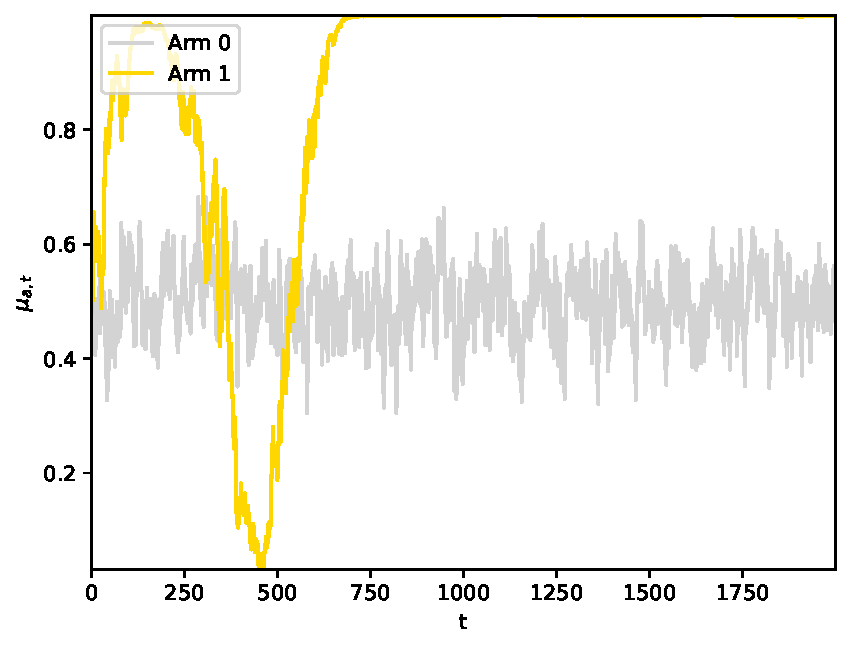
\includegraphics[width=\textwidth]{./fods_figs/dynamic/logistic/dynamics_c}
		\caption{Expected per-arm rewards over time for Scenario C in Equation~\eqref{eq:linear_mixing_dynamics_c}.
			Notice the early optimal arm change at $t\approx600$.
		}
		\label{fig:linear_mixing_dynamics_c_logistic}
	\end{subfigure}\qquad
	\begin{subfigure}[b]{0.45\textwidth}
		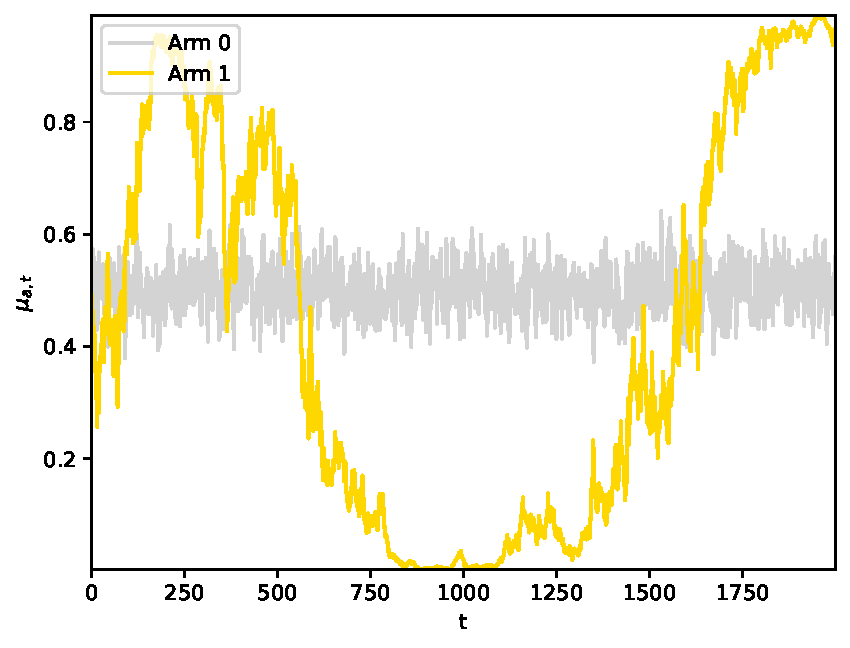
\includegraphics[width=\textwidth]{./fods_figs/dynamic/logistic/dynamics_d}
		\caption{Expected per-arm rewards over time for Scenario D in Equation~\eqref{eq:linear_mixing_dynamics_d}.
			Notice the late optimal arm change at $t\approx1650$.
		}
		\label{fig:linear_mixing_dynamics_d_logistic}
	\end{subfigure}
	
	\begin{subfigure}[b]{0.47\textwidth}
		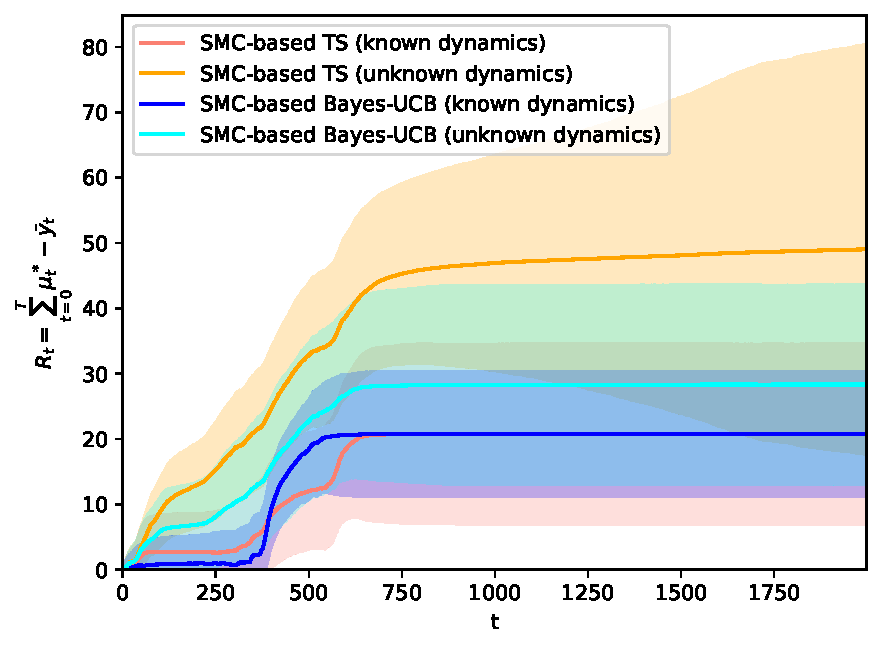
\includegraphics[width=\textwidth]{./fods_figs/dynamic/logistic/c_M2000_cumulative_regret_dunknown}
		\caption{Cumulative regret for SMC-based Bayesian policies in scenario C: known and unknown dynamic parameters.}
		\label{fig:dynamic_bandits_c_logistic_cstatic}
	\end{subfigure}\qquad
	\begin{subfigure}[b]{0.47\textwidth}
		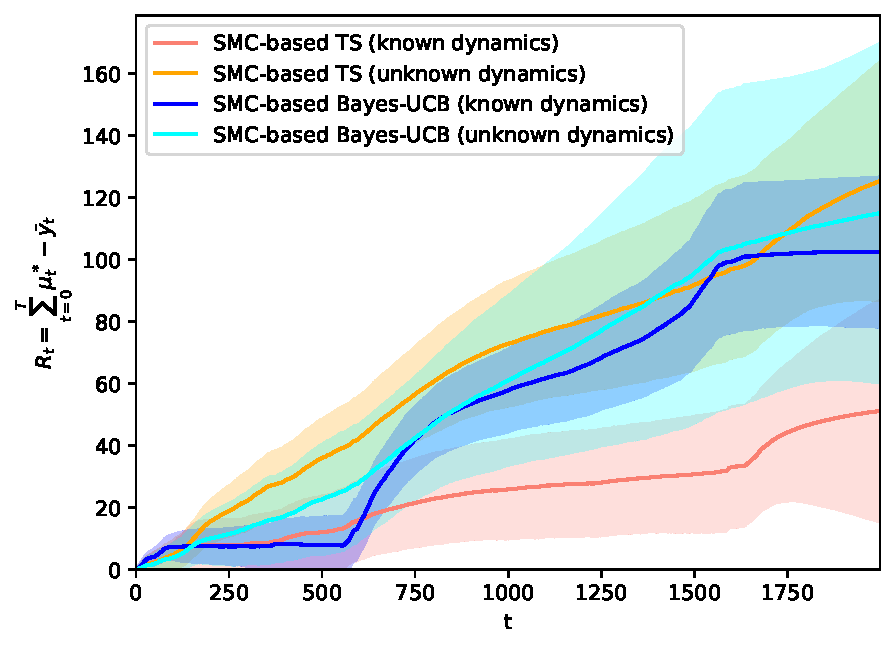
\includegraphics[width=\textwidth]{./fods_figs/dynamic/logistic/d_M2000_cumulative_regret_dunknown}
		\caption{Cumulative regret for SMC-based Bayesian policies in scenario D: known and unknown dynamic parameters.}
		\label{fig:dynamic_bandits_d_logistic_cstatic}
	\end{subfigure}
	\caption{
		Mean regret (standard deviation shown as shaded region) in contextual linear logistic dynamic bandit Scenarios C and D
		described in Equations~\eqref{eq:linear_mixing_dynamics_c}--\eqref{eq:linear_mixing_dynamics_d}.
		Notice the difference in early ($t\approx600$ in Scenario C) and late ($t\approx1650$ in Scenario D) optimal arm changes,
			as illustrated in Figures~\ref{fig:linear_mixing_dynamics_c_logistic}--\ref{fig:linear_mixing_dynamics_d_logistic},
		and their impact in regret,
			as showcased in Figures~\ref{fig:dynamic_bandits_c_logistic_cstatic}--\ref{fig:dynamic_bandits_d_logistic_cstatic}.
		SMC-based Bayesian policies adapt and find the right exploration-exploitation tradeoff.}
	\label{fig:dynamic_bandits_logistic}
\end{figure}
